\documentclass[12pt]{article}
\usepackage[a4paper, margin=2cm]{geometry}
\usepackage[english]{babel} % To obtain English text with the blindtext package
\usepackage{blindtext}
\usepackage{graphicx} % Required for inserting images
\usepackage{array, multirow} % For extra column formatting
\usepackage{amsmath, amssymb} %for equation environment
\usepackage{float}
\usepackage{parskip, } % For gaps between para
\usepackage{setspace}
\usepackage{pdfpages}
\usepackage{abstract}
\usepackage[export]{adjustbox}
\usepackage{emptypage}
\usepackage{tocloft}
\usepackage[nottoc]{tocbibind}
\usepackage{hyperref, url}
\usepackage{subcaption}
\usepackage{lipsum}
\usepackage[table]{xcolor}
\usepackage{caption}
    \captionsetup{font=footnotesize,labelfont=bf}

\cftsetindents{section}{0em}{2em}
\cftsetindents{subsection}{0em}{2em}

\renewcommand\cfttoctitlefont{\hfill\Large\bfseries}
\renewcommand\cftaftertoctitle{\hfill\mbox{}}

\graphicspath{ {./images/} }

\pagenumbering{arabic}

\definecolor{blurple}{HTML}{5865F2}

\hypersetup{
    colorlinks=true,
    linkcolor=black,
    urlcolor=blurple,
    citecolor=blurple,
}

\urlstyle{same}

\renewcommand{\arraystretch}{1.3}

\setcounter{secnumdepth}{5}
\setcounter{tocdepth}{5}
\newcommand\simpleparagraph[1]{%
  \stepcounter{paragraph}\paragraph*{\theparagraph\quad{}#1}}

%%%%%%%%%%%%%%%%%%%%%%%%%%%%%%%%%%%


\title{PHYC20040 Exp.2 Pleiades SM}
\author{Joana Adao}
\date{\today}

\begin{document}

\begin{titlepage}
    \begin{center}

        \begin{figure}[ht]
            
\includegraphics[width=\textwidth]{UCDLogo.png}
        \end{figure}
        
        \begin{figure}
            \centerline{
\includegraphics[width=\paperwidth]{UCDBanner.png}}
        \end{figure}

        \vspace{4cm}

        {\LARGE \bfseries PHYC20040 Exploring the Solar System}\\
        \vspace{0.75cm}
        {\Large Experiment No.2 Photoelectric Photometry of the Pleiades}
        
        \vspace{1cm}
    
    {\Large \textbf{12 February 2025}}

    \vspace{2cm}
    
    {\large \textbf{by Joana C.C. Adao (Student No. 23311051)}}\\

    \end{center}
    
   \clearpage

\end{titlepage}

\setcounter{page}{1}
\tableofcontents

\newpage

\begin{abstract}
\addcontentsline{toc}{section}{Abstract}

\vspace{1cm}

The aim of this experiment was 

\end{abstract}

%%%%%%%%%%%%%%%%%%%%%%%%%%%%%%%%%%%

\section{Theory} \label{sec:1}

Photometry 

\subsection{Photometry} \label{sec:1.1}

\textbf{Photometry} is a measurement of the brightness of celestial objects, such as stars and planets, that give astronomers access to that celestial object's composition,
temperature, distance, age, and more
\cite{britphoto}.
It is a special subset of radiometry which measures light waves by the typical response of the average human eye
\cite{mictechphoto, photophoto}.

Photometry has some fundamental quantities that aid in understanding what is being measured \cite{WYATT197815,photophoto}:

\begin{itemize}
    \item \textbf{Luminous flux} is the visible light per second that the source radiates. It is measured with \textit{lumens} given by \textit{Watts}.
    \item \textbf{Luminous intensity}, directly related to the luminous flux, is the lumens per unit solid angle emitted. Originally known as 'candlepower', the unit of measurement
    is \textit{candela} given by \textit{Watts per steradian}.
    \item \textbf{Illuminance} is the measurement of the level of light at a particular surface. The unit of measurement is \textit{footcandle (English)} or \textit{lux (Metric)} which is
    given by \textit{Watts per square metre}.
    \item \textbf{Luminance} is what measures the apparent magnitude (brigthness) (see §\ref{sec:1.1.3}), it is the luminous flux that is emitted from a surface.
    It is therefore measured with the unit \textit{footlambert (English)} or \textit{candela per square metre (Metric)}, given be \textit{Watt/steradian/}$m^2$.
    The human eye is the most commonly-known luminance detector, of which the sensitivity to light, and therefore colour, can be seen in figure {\ref{fig:1}}.
\end{itemize}

\begin{figure}[H]
    \centering
    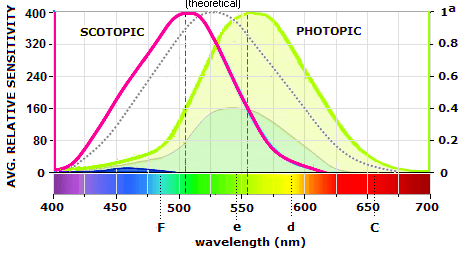
\includegraphics[width=12.5cm]{eye spectra curve.png}
    \caption{\centering Curve of the spectral sensitivity of the human eye \protect\cite{eyecurve}. \textit{Scotopic: very low light levels; Photopic: bright light levels \protect\cite{scophoto}.}}
    \label{fig:1}
\end{figure}

\subsubsection{UBV Photometry} \label{sec:1.1.1}



\subsubsection{The B-V Colour Index} \label{sec:1.1.2}



\subsubsection{Apparent and Absolute Magnitude} \label{sec:1.1.3}

Magnitude is a measure of the brightness of a star or other celestial body. The brighter the object, the lower the magnitude (number)
\cite{britmag}.
The magnitude of the celestial objects are divided into two types of observation:

\begin{itemize}
    \item \textbf{Apparent magnitude, m,} is used to describe how bright a celestial object appears from the view on Earth. Some of the brightest objects we can see
    have \textit{negative} apparent magnitude values (Sun = -26.7, Pluto (at brightest) = +13.7, for reference), meaning that they are particularly bright.
    \cite{lcomag}.
    \item \textbf{Absolute magnitude, M,} is defined as the magnitude of the star if the distance between it and Earth were 10 parsecs (pc)
    \cite{lcoabsmag,cosmosabsmag}.
    When at a set distance, astronomers are then able to compare intrinsic brightness of stars. The absolute magnitude refers to the absolute 'visual' magnitude, which restricts
    the measurement of the brightness to wavelength (4000 - 7000 Å)
    \cite{cosmosabsmag}.
    These magnitudes can also be negative values for particularly bright stars.
\end{itemize}

Absolute (\textbf{M}) and apparent (\textbf{m}) magnitudes can be used using equation \ref{eq:1} to calculate \textbf{D}, the distance in parsecs (pc). The magnitudes do not have units.
The distance modulus is then $\mathbf{m - M}$
\cite{cosmosabsmag}.

\begin{gather} \label{eq:1}
    M = m + 5 - 5 (\log_{10} D) \quad , \quad m - M = 5 \log_{10} \left( \frac{D}{10} \right)
\end{gather}

The above equation (\ref{eq:1}) can be manipulated to find the distance, \textbf{D}:

\begin{gather} \label{eq:2}
    \log_{10}D = \frac{m - M + 5}{5} \quad \implies \quad D = 10^{\frac{m - M + 5}{5}}
\end{gather}

\paragraph{The Link Between Magnitude and Photometry}



\subsection{Hertzsprung-Russel (H-R) Diagram}



\subsubsection{Main Sequence Stars}



\subsection{The Pleiades Star Cluster}



\section{Methodology} \label{sec:2}



\section{Results and Calculations} \label{sec:3}



\section{Conclusion} \label{sec:4}



\newpage

%%%%%%%%%%%%%%%%%%%%%%%%%%%%%%%%%%%

\bibliographystyle{IEEEtran}
\bibliography{References} \label{sec:ref}

\newpage

\section*{Appendix} \label{sec:A}
\addcontentsline{toc}{section}{Appendix}

\subsection*{Code}
\addcontentsline{toc}{subsection}{Code}


\listoffigures

\listoftables

\end{document}